\newgeometry{executivepaper,left=1.3cm,right=1.3cm,top=1.5cm,bottom=1.5cm,footskip=.5cm}

\setlength{\columnsep}{1.5cm}
\pagestyle{fancyplain}
\fancyhf{}
\fancyfoot[R]{45}

\begin{multicols}{2}

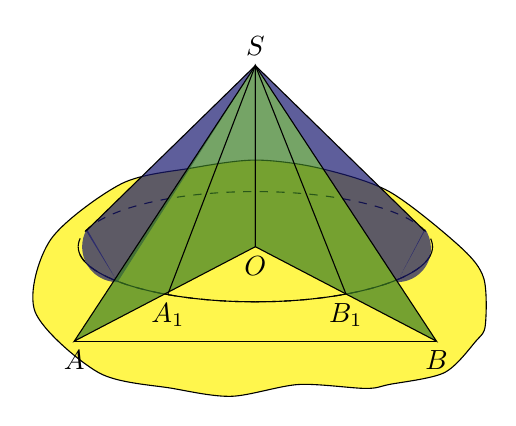
\begin{tikzpicture} 
    \coordinate (a) at (3, 0);
    \coordinate (b) at (2.2, -0.1);
    \coordinate (c) at (1.3, -0.3);
    \coordinate (d) at (0.4, -1.01);
    \coordinate (e) at (0.2, -1.92);
    \coordinate (f) at (1.01, -2.7);
    \coordinate (f1) at (1.95, -2.9);
    \coordinate (g) at (2.7, -3);
    \coordinate (g1) at (3.55, -2.85);
    \coordinate (h) at (4.4, -2.9);
    \coordinate (i) at (4.7, -2.85);
    \coordinate (i1) at (5.4, -2.7);
    \coordinate (j) at (5.8, -2.3);
    \coordinate (k) at (5.92, -2.1);
    \coordinate (l) at (5.9, -1.5);
    \coordinate (m) at (5.6, -1.1);
    \coordinate (n) at (4.7, -0.4);
    \coordinate (o) at (3.8, -0.1);
    
    \filldraw[fill=yellow!70, draw=black] plot[smooth cycle] coordinates {(a) (b) (c) (d) (e) (f) (f1) (g) (g1) (h) (i) (i1) (j) (k) (l) (m) (n) (o)};

    \def\xR{2.25}; %x radius of ellipse
    \def\yR{0.7};  %y radius of ellipse
    \draw [dashed] (3, -1.1) ellipse ({\xR} and {\yR});
    \draw (-\xR+3,-1.1) arc[start angle=180,end angle=360,x radius=\xR,y radius=\yR]; %bottom half

    \draw (0.7, -2.3) -- (5.3, -2.3);

    \fill[fill opacity=0.7, fill=MidnightBlue] (3, 1.2) -- (0.85, -0.9) -- (1.25, -1.55) -- cycle;

    \fill[fill opacity=0.7, fill=MidnightBlue] (1.25, -1.55) arc(270:150:0.45);

    \fill[fill opacity=0.7, fill=MidnightBlue] (3, 1.2) -- (5.15, -0.9) -- (4.8, -1.55) -- cycle;

    \fill[fill opacity=0.7, fill=MidnightBlue] (4.8, -1.55) arc(270:395:0.43);

    \filldraw[text opacity=1, fill opacity=0.7, fill=OliveGreen, draw=black] (0.7, -2.3) node[anchor=north]{$A$}
        -- (3, -1.1) node[anchor=north]{$O$}
        -- (3, 1.2) node[anchor=south]{$S$}
        -- cycle;
    \filldraw[text opacity=1, fill opacity=0.7, fill=OliveGreen, draw=black] (5.3, -2.3) node[anchor=north]{$B$}
        -- (3, -1.1) node[anchor=north]{}
        -- (3, 1.2) node[anchor=south]{}
        -- cycle;

    \draw (3, 1.2) -- (0.85, -0.9);
    \draw (3, 1.2) -- (5.15, -0.9);

    \draw (3, 1.2) -- (1.89, -1.7) node[anchor=north]{$A_1$};
    \draw (3, 1.2) -- (4.15, -1.7) node[anchor=north]{$B_1$};

    
\end{tikzpicture}
\\
\\
$\varangle O S B=\beta, \varangle O S A_1=\varangle O S B_1=\varphi$. 
Вычислим косинус угла $A_1 O B_1$, являющегося линейным углом двугранного угла, образованного плоскостями треугольников $O S A$ и $O S B$. Для этого найдем $A_1 B_1^2$ по теореме косинусов из треугольника $A_1 S B_1$ и из треугольника $A_1 O B_1$, а затем приравняем полученные выражения. Получим
$$
\begin{aligned}
        & A_1 S^2+B_1 S^2-2 A_1 S \cdot B_1 S \cdot \cos x= \\
        & =A_1 O^2+B_1 O^2-2 A_1 O \cdot B_1 O \times \\
        & \times \cos \varangle A_1 O B_1 .
\end{aligned}
$$

Так как $A_1 S^2=S O^2+A_1 O^2, B_1 S^2 =S O^2+B_1 O^2$, то отсюда следует
$$
\begin{aligned}
        & 2 A_1 O \cdot B_1 O \cdot \cos \measuredangle A_1 O B=2 A_1 S \times \\
        & \times B_1 S \cdot \cos x-2 O S^2 .
\end{aligned}
$$
Подставим в это выражение $A_1 O = B_1 O=O S \cdot \operatorname{tg} \varphi, A_1 S=B_1 S=\frac{OS}{\cos \varphi}$ и после сокращения на $2  OS^2$ получим
$$
\begin{aligned}
    \operatorname{tg}^2 \varphi \cdot \cos \varangle A_1 O B_1=\frac{\cos x}{\cos ^2 \varphi}-1 \text { или }
\end{aligned}
$$
\begin{equation}
    \label{eq:1}
    \cos \varangle A_1 O B_1=\frac{\cos x-\cos ^2 \varphi}{\sin ^2 \varphi} \text{.}
\end{equation}
Из треугольников $ASB$ и $AOB$ имеем 
\begin{equation}
    \label{eq:2}
    \cos \varangle A O B=-\operatorname{ctg} \alpha \operatorname{ctg} \beta \text{.}
\end{equation}
Так как $\varangle AOB=\varangle A_1 O B_1$, то, приравнивая правые части равенств (\ref{eq:1}) и (\ref{eq:2}), получим
$$
\cos x=\cos ^2 \varphi-\sin ^2 \varphi \operatorname{ctg} \alpha \operatorname{ctg} \beta,
$$
откуда окончательно:
$$
x=\arccos \left(\cos ^2 \varphi-\sin ^2 \varphi \operatorname{ctg} \alpha \operatorname{ctg} \beta\right) .
$$

С этой задачей справились немногне поступавшие.

Заметим, что формулы (\ref{eq:1}) и (\ref{eq:2}) выражают зависимость между внутренним двугранным углом и плоскими углами при вершине трехгранного угла. В общем случае, если $A, B$ и C --- внутренние двугранные углы, противолежащие соответственно плоским углам $\alpha, \beta$ и $\gamma$ трехгранного угла, то справедливы формулы:
$$
\begin{aligned}
& \cos A=\frac{\cos \alpha-\cos \beta \cos \gamma}{\sin \beta \sin \gamma}, \\
& \cos B=\frac{\cos \beta-\cos \alpha \cos \gamma}{\sin \alpha \sin \gamma}, \\
& \cos C=\frac{\cos \gamma-\cos \alpha \cos \beta}{\sin \alpha \sin \beta},
\end{aligned}
$$
которые выводятся так же, как и формула (\ref{eq:1}). Эти формулы могут оказаться полезными при решении многих стереометрических задач.

В заключение предлагаем самостоятельно решить следующий вариант, предлагавшийся на письменном экзамене.

    \begin{center}
        \textcolor{cyan}{Вариант 1}
    \end{center}
    
    \textbf{1.} Определить все действительные значения $a$, при каждом из которых уравнение
    $$
    \cos ^4 x-(a+2) \cos ^2 x-(a+3)=0 \\
    $$
    имеет решения, и найти все эти решения.
    
    \textbf{2.} Решить уравнение
    $$
    \left|1-\log _{\frac{1}{6}} x\right|+2=\left|3-\log _{\frac{1}{6}} x\right| .
    $$
    
    \textbf{3.} Из города $A$ в город $B$, находящийся на расстоянии 105 \textit{км} от $A$, с постоянной скоростью $v$ \textit{км/ч} выходит автобус. Через 30 \textit{мин} вслед за ним из $A$ со скоростью $40$ \textit{км/ч} выезжает автомобиль, который, догнав в пути автобус, поворачивает обратно и движется с прежней скоростью. Oпределить все те значения $v$, при которшх автомобиль возвращается в $A$ позже, чем автобус приходит в $B$.
    
    \textbf{4.} В треугольнике $A B C$ сторона $B C$ служит основанием полукруга, площадь которого равна площади треугольника $A B C$. Угол $A$ равен $\alpha$. Найти углы $B$ и $C$, считая, что $B \geqslant C$. Исследовать, при каких значениях угла $\alpha$ задача имеет решение.
    
    \textbf{5.} В прямом круговом конусе с вершиной $S$ угол между образуоними $S A$ и $S B$ равен $\alpha$, а угол между их проекциями на плоскость основания равен $\beta$. Вычислить угол между биссектрисами углов $O S A$ и $O S B$, где точка $O$ является центром круга, служащего основанием конуса.

\end{multicols}